\chapter{Background and Motivation}
\label{section:background}

\section{Recent Trends}

\parikshan is driven by some recent trends in the industry towards faster bug resolution and quicker development, and scaled deployment.
In this section we discuss three such trends in the industry which are of particular relevance to \parikshan.

\subsection{Software development trends}

Software development paradigms have evolved over the years from a more documentation oriented process to quicker and faster releases. The software development industry is working towards faster evolving softwares, rather than building monolithic softwares for long term uses.
Similarly software development no longer follows strict regimented roles of developer, administrator/operator, tester etc, instead new paradigms are being developed which encourage cross-functionalities.

One recent trend in software development processes is \emph{agile}~\cite{agile} and \emph{extreme}~\cite{extremeProgramming} programming development paradigms. Compared to traditional \emph{waterfall model}~\cite{waterfall}, both \emph{agile} and \emph{extreme} programming focus on faster response to changing customer demands, and a quicker delivery time. Agile programming for instance works on the principle of very short development cycles called -\emph{scrums}. At the end of each scrum, there should be a working software product that can be readily deployed. The work-items are generally short, and goal oriented, and a scrum will usually last at most 2 weeks. 

Agile development focuses on shorter development cycle, to apply patches, bug-fixes and having a leaner team/operations.
\parikshan's live-debugging capability is yet another tool to facilitate faster software development and debugging, by allowing developers to debug their applications in parallel to the one deployed in production.
We believe agile development can be tied up with \parikshan to have an end-to-end quick test, debug, and deploy strategy and make application development an even more lean process.

\begin{figure*}[!ht]
	\begin{center}
		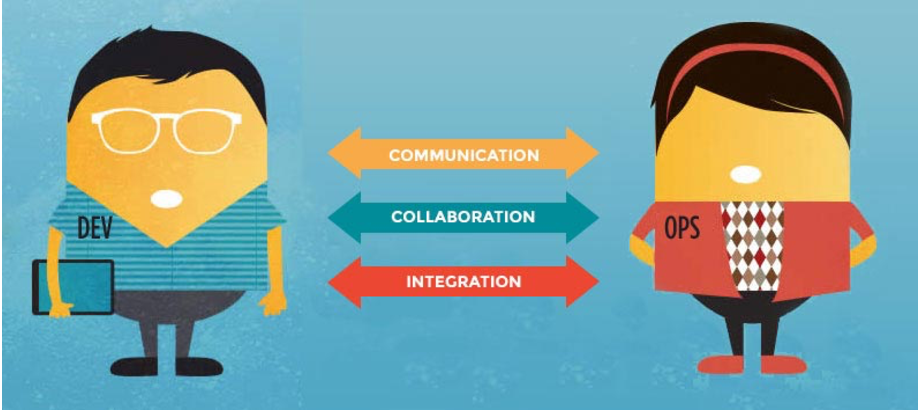
\includegraphics[width=0.8\textwidth]{guided/figs/devops.pdf}
		\caption{Devops software development process}
		\label{fig:devops}
	\end{center}
\end{figure*}

Another trend in software development is cross-functional development and production application management called \emph{Devops}~\cite{10DevOps}.
\emph{Devops} is a term used to refer to a set of practices that emphasizes the collaboration and communication of both software developers and other information-technology (IT) professionals (operators/administrators) while automating the process of software delivery and infrastructure changes.
The key in devops is the close collaboration of developers and operators, and an interchangable role (i.e. developers are also operators for real-time critical systems), or alternatively having developers and operators being active in the entire software cycle (including QA and operations).
The old view of operations tended towards the “Dev” side being the “makers” and the “Ops” side being the “people that deal with the creation after its birth” – the realization of the harm that has been done in the industry of those two being treated as siloed concerns is the core driver behind DevOps.

The driving force behind this change, where expensive resources(developers), are applied on what is traditionally managed by operators(with lower expertise or understanding of the software) - is to have faster responses and a shorter time to debug.
This necessity of having a shorter time to debug, and the availability of developers in the operation stage is one of the trend which motivates live debugging. 
Clearly developers who have much better understanding of the source code (having written it themselves), will be able to debug the application faster as long as they have some degree of visibility and debug-capability within the application.
We believe that \parikshan's livedebugging framework will allow such developers to debug their application in an isolated yet parallel environment, which clones in real-time the behavior without impacting the production.
This will greatly reduce development overhead by giving crucial insight and make the feedback cycle shorter.
\emph{This will shorten the time to debug, and will easily fit into a debugging paradigm in an already increasing trend of devops.}.


\subsection{Microservice Architecture}

\begin{figure*}[h!]
	\begin{center}
		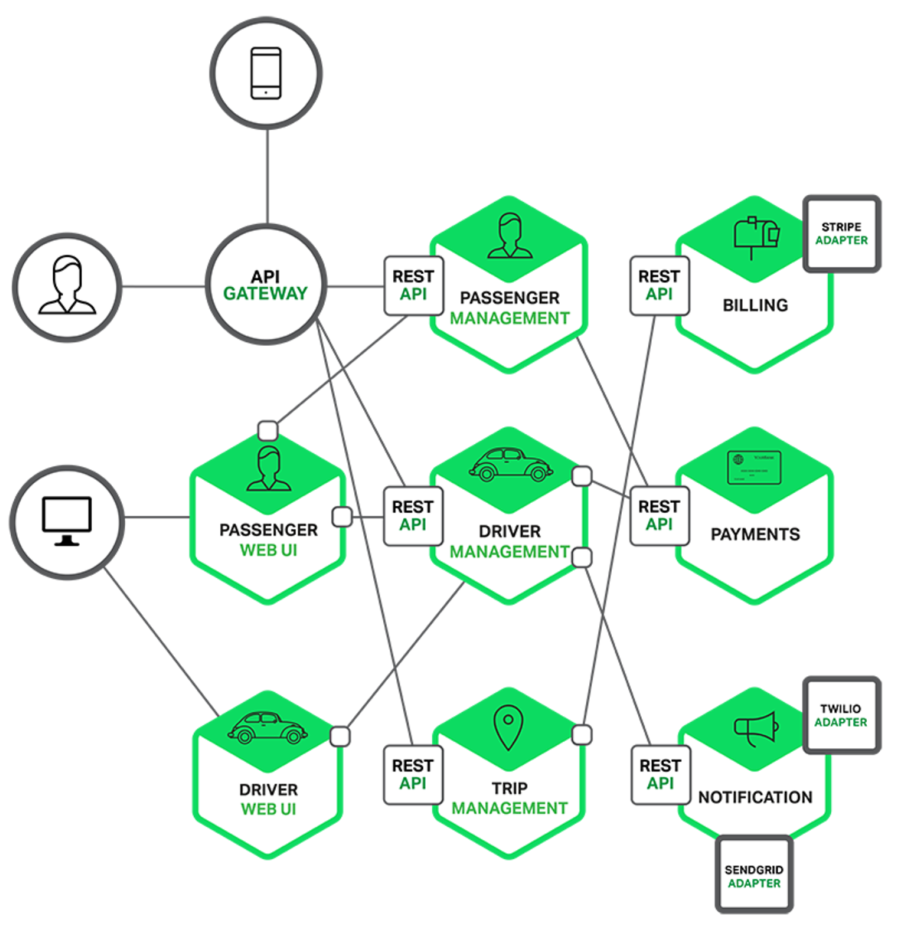
\includegraphics[width=0.8\textwidth]{guided/figs/microservice.pdf}
		\caption{An example of a microservice architecture for a car renting agency website}
		\label{fig:microservice}
	\end{center}
\end{figure*}

As applications grow in size they grow more and more complex with several interacting modules. 
With iterative improvements in every release applications tend to grow in code-size with large obsolete code-bases, un-productive technology, and which is difficult to maintain or modify owing to it's size and complexity.
Many organizations, such as Amazon, eBay, and Netflix, have solved this problem by adopting what is now known as the Microservices Architecture pattern. Instead of building a single monstrous, monolithic application, the idea is to split your application into set of smaller, interconnected services.

A service typically implements a set of distinct features or functionality, such as order management, customer management, etc. Each microservice is a mini-application that has its own hexagonal architecture consisting of business logic along with various adapters. Some microservices would expose an API that’s consumed by other microservices or by the application’s clients. Other microservices might implement a web UI. At runtime, each instance is often a cloud VM or a Docker container.

Figure ~\ref{fig:microservice} shows the micro-service architecture of a car renting agency website.
Each functional area is implemented as it's own independent service.
Moreover, the web application is split into a set of simpler web applications (such as one for passengers and one for drivers in our taxi-hailing example). This makes it easier to deploy distinct experiences for specific users, devices, or specialized use cases.


\subsection{Virtualization, Scalability and the Cloud}
\label{sec:backVirtualization}

Modern day service oriented applications, are large and complex systems, which can serve billions of users. Facebook has 1.79 billion active users every month, and Google search has approximately 1.71 billion users, similarly twitter, netflix, instagram, and several other such websites have a huge base of users. 

\xxx{Cloud and virtualization is common place and is used for deployment of most modern day services. This allows for our assumption of plethora of resource, as well as a deployment infrastructure already focused on execution in isolation. One of the core ideas behind \livedebugging}

\section{Current debugging of production systems}
\label{sec:backCurrentStatus}

Before moving forward with a new software debugging paradigm, we want to discuss the current state-of-art debugging mechanisms followed in the industry. The software development cycle consists of the following four components - software development, monitoring, modeling \& analytics, and software debugging. 

Here monitoring involves getting periodic statistics or insight regarding the application, when deployed in the production environment, either using instrumentation within the application or using periodic sampling of resource usage in the system.
Monitoring gives an indication regarding the general health of the system, and can alert the user incase anything has gone wrong. 
System level default tools provided by most commodity operating systems, like process monitors in linux, mac and windows, provide a high level view of real-time resource usage in the system.
On the other hand, software event monitoring tools like nagios, ganglia, and rsyslog ~\cite{nagios,ganglia,rsyslog} aggregate logs and provide a consolidated view of application operations a cluster of machines to the administrator. 
On the other hand, tools like SystemTap~\cite{systemtap}, DTrace~\cite{dtrace} allow operators to write customized instrumentation and dynamically patch them into applications to allow for a much deeper understanding of the system (albeit at higher overheads).

Modeling and analytics is generally a follow up step, which uses the output of monitoring and can provide useful insights using the monitoring data in real-time to highlight outliers and unexpected behavior.
Tools like loggly~\cite{loggly}, ELK~\cite{elk}, Splunk~\cite{splunk}, allow operators to search logs in real-time, as well as provide statistical analytics for different categories of logs.
Academic tools like vpath~\cite{vpath}, magpie~\cite{magpie}, spectroscope~\cite{spectroscope}, appinsight~\cite{appinsight}, amongst others can stitch events together to give a much more detailed transaction flow analysis.

\begin{figure*}[h!]
	\begin{center}
		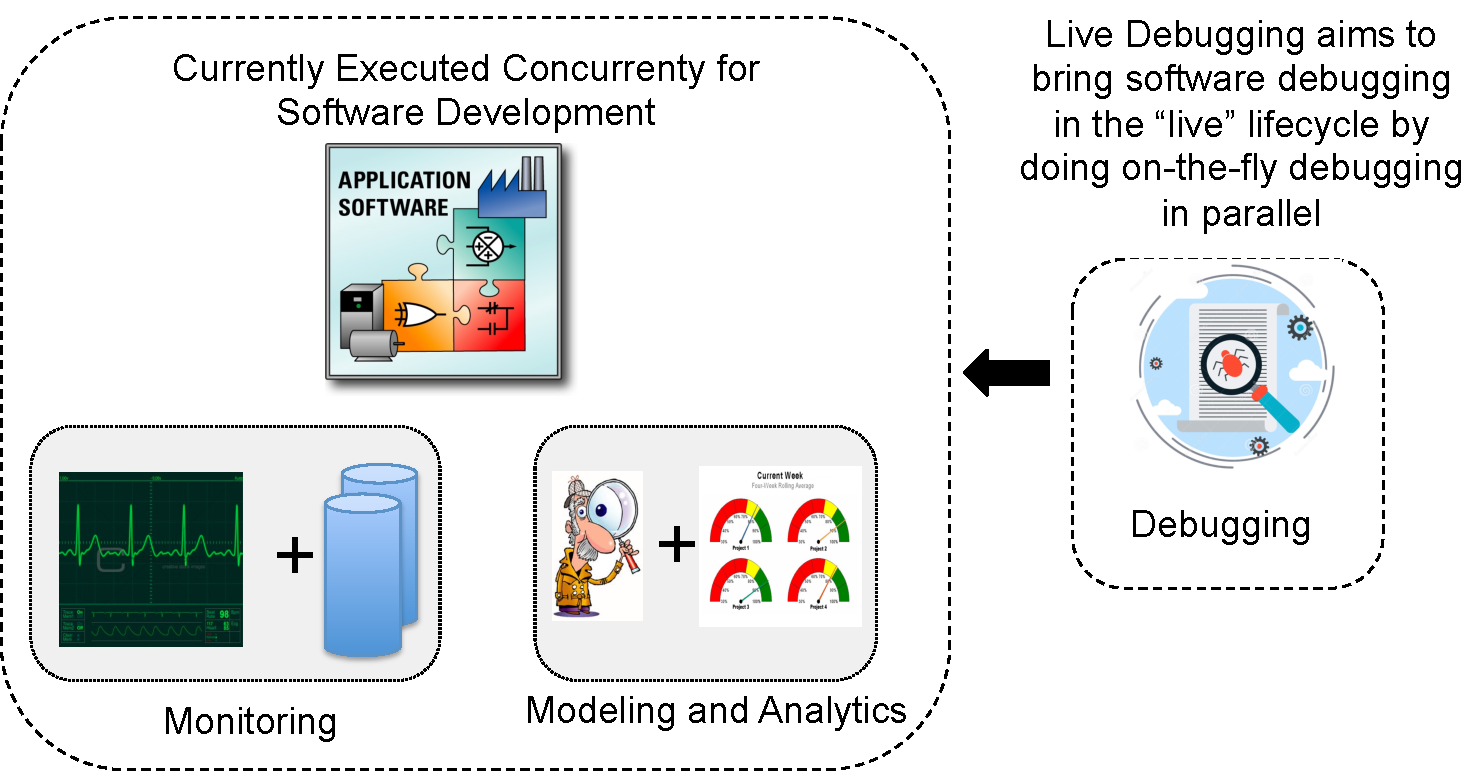
\includegraphics[width=0.95\textwidth]{intro/livedebuggingTrends.pdf}
		\caption{Live Debugging aims to move debugging part of the lifecycle to be done in parallel to the running application, as currently modeling, analytics, and monitoring is done}
		\label{fig:liveDebugTrends}
	\end{center}
\end{figure*}


As can be seen in figure~\ref{fig:liveDebugTrends}, 
both monitoring and analytics happen in real-time in parallel to production applications. However, without any interaction with the running application these techniques are only limited to realizing that the production system has a bug, and potentially localizing the error.
The actual root-cause extraction unfortunately currently relies on offline debugging.
\parikshan aims to move the debugging process from an offline process to a completely or partially online (real-time) process in order to shorten time to debugging.
In some cases our framework can also be used for patch testing and fix validation.
In the next section we will see a real-world motivation scenario for \parikshan.



\section{Motivating Scenario}
\label{sec:motivation}

Consider the complex multi-tier service-oriented system shown in Figure \ref{fig:motivation} that contains several interacting services (web servers, application servers, search and indexing, database, etc.). 
The system is maintained by operators who can observe the health of the system using lightweight monitoring that is attached to the deployed system.
\xxx{Still need some statement here that it's reasonable to assume that they are already running each tier in its own container... This is an important one...}
%In the interest of application performance, production system monitoring is usually limited to system resource usage, application usage statistics, transaction logs, and error logs.
At some point, an unusual memory usage is observed in the glassfish application server, and some error logs are generated in the Nginx web server. 
Administrators can then surmise that there is a potential memory leak/allocation problem in the app-server or a problem in the web server.
However, with a limited amount of monitoring information, they can only go so far.


Typically, trouble tickets are generated for such problems, and they are debugged offline.
However using \parikshan, administrators can generate replicas of the Nginx and Glassfish containers as \textbf{\textit{Nginx-debug}} and \textbf{\textit{glassfish-debug}}.
\parikshan's network duplication mechanism ensures that the debug replicas receive the same inputs as the production containers and that the production containers continue to provide service without interruption.
This separation of the production and debug environment allows the operator to use dynamic instrumentation tools to perform deeper diagnosis without fear of additional disruptions due to debugging.
Since the replica is cloned from the original potentially ``buggy'' \productioncontainer, it will also exhibit the same memory leaks/or logical errors.
Additionally, \parikshan can focus on the ``buggy'' parts of the system, without needing to replicate the entire system in a test-cluster.
This process will greatly reduce the time to bug resolution, and allow real-time bug diagnosis capability.

The replica can be created at any time: either from the start of execution, or at any point during execution that an operator deems necessary, allowing for post-facto analysis of the error, by observing execution traces of incoming requests (in the case of performance bugs and memory leaks, these will be persistent in the running system).
Within the debug replica, the developer is free to employ any dynamic analysis tools to study the buggy execution, as long as the only side-effect those tools is on execution speed.
%\xxx{need to describe assumptions: debug is identical except for external timing/slowdowns (need to clarify what kind of debugging activities are permitted). assume that it's OK to use a VM as the container, and that it is 'free' to dos so}

\begin{figure*}[ht!]
	\begin{center}
		%    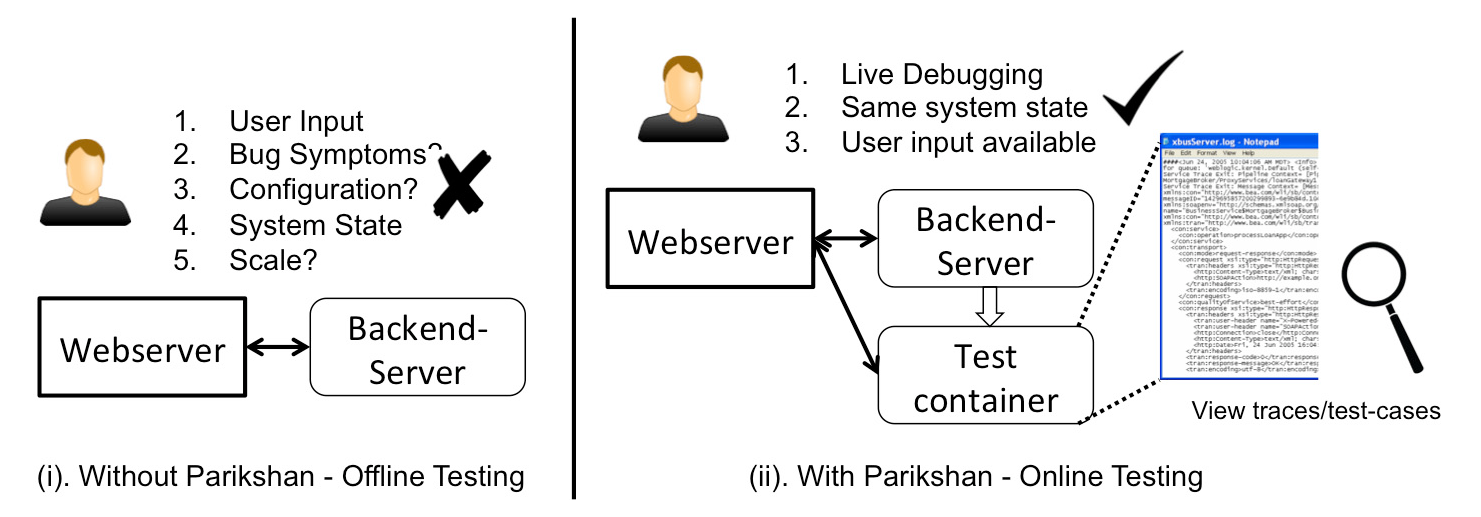
\includegraphics[width=0.7\textwidth]{figs/motivation.eps}
		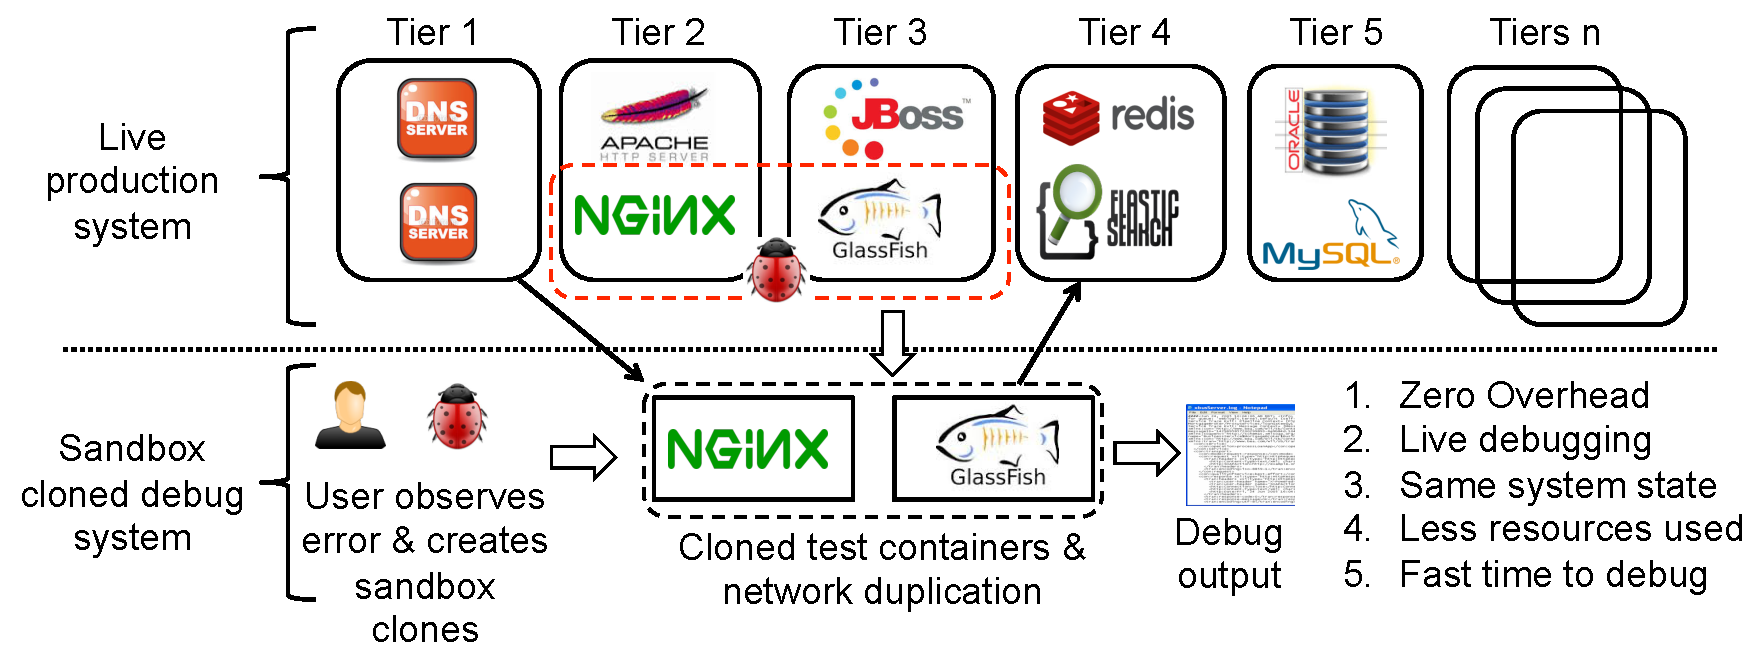
\includegraphics[width=0.99\textwidth]{parikshan/figs/workflow3.pdf}
		\caption{Workflow of \parikshan in a live multi-tier production system with several interacting services. When the administrator of the system observes errors in two of it's tiers, he can create a sandboxed clone of these tiers and observe/debug them in a sandbox environment without impacting the production system.}
		\label{fig:motivation}
	\end{center}
\end{figure*}

\section{Summary}

In this chapter we first discussed some recent software trends which motivated the development of \parikshan, and show that it complements as well as is driven by the current direction of industry. 
We then discussed the current state-of-art practices followed in the industry for most production applications, and showed the current limitation in doing real-time debugging.
We then discussed a motivation scenario highlighting a real-world use-case for \parikshan, and how livedebugging could hypothetically take place.


\xxx{In this chapter we }